\documentclass[runningheads]{llncs}
\usepackage[T1]{fontenc}
\usepackage{graphicx}
\usepackage{amsmath,amssymb}
\usepackage{booktabs}
\usepackage{xcolor}
\usepackage{hyperref}
\usepackage{algorithm}
\usepackage{algpseudocode}
% \usepackage[utf8]{inputenc}
\usepackage{todonotes}
\usepackage{siunitx}
\usepackage{subcaption}
\usepackage{tikz}
\usepackage{multicol}
\usepackage{float}

\begin{document}

\title{Motzkin Neighborhood Evaluation in Tabu Search
and Simulated Annealing for the Permutational
Flow Shop Problem}

\titlerunning{Motzkin Neighborhood Evaluation}


\author{Remigiusz Wojewódzki\inst{1} \and Wojciech Bożejko\inst{2}}
\authorrunning{R. Wojewódzki, W. Bożejko}

\institute{
Wrocław University of Science and Technology, Poland\\
\email{remigiusz.wojewodzki@gmail.com}
\and
Wrocław University of Science and Technology, Poland\\
\email{wojciech.bozejko@pwr.edu.pl}
}
\maketitle           

\begin{abstract}
In this paper, we investigate the impact of using the \emph{Motzkin} neighborhood in the permutation flow shop problem (PFSP) for two metaheuristic scheduling algorithms: Tabu Search and Simulated Annealing. The goal is to minimize $C_{\max}$, understood as the completion time of all jobs. The Motzkin neighborhood enables performing multiple swaps of permutation elements during a single iteration, i.e., simultaneous swaps of multiple permutation elements with allowed nesting, while prohibiting crossings of the lines connecting the elements. The use of dynamic programming reduces the computational complexity and speeds up the algorithm. In this paper, we compare the \emph{Motzkin} neighborhood with the \emph{Fibonacci} neighborhood and the classical \emph{Dynasearch} and \emph{Adjacent} neighborhoods. The experiments were conducted on Taillard benchmark instances for many different time limits. The obtained results allow us to conclude that the choice of neighborhood has a significant impact on the quality of the result obtained by the algorithm within the given time. For all investigated time limits, \emph{Dynasearch} achieved the best results (the smallest average gap), while the \emph{Fibonacci} neighborhood is at the other end of the ranking. The \emph{Motzkin} neighborhood examined in detail in this work is, in most cases, ranked better than \emph{Adjacent}. This advantage becomes clearly visible for larger allowed computation times. The obtained results suggest that neighborhoods using multi-swap moves constitute an interesting alternative to their classical (simpler) counterparts, noting that further computational optimization of complex neighborhoods is required.

\keywords{Flow shop scheduling \and Metaheuristics \and Tabu search \and Simulated annealing \and Composite neighborhood \and Motzkin}
\end{abstract}

\section{Introduction}
The Permutation Flow Shop Problem (PFSP), mathematically defined in \cite{ref_bozejko_parallel}, consists of finding a permutation of $n$ jobs processed on $m$ machines in the same order. The objective is to minimize the completion time of all jobs (makespan) $C_{\max}$. The problem is known to be NP-hard for $m \ge 3$, which motivates the use of metaheuristic methods. In metaheuristic algorithms, the neighborhood of a solution $x$ is defined as the set of solutions that can be obtained through admissible modifications of $x$ \cite{vanlaarhoven1992}.

In addition to the choice of the general algorithm, the selection of the neighborhood structure is equally important. In the classical approach, neighborhood elements perform simple moves, which results in the solution space being explored locally and relatively shallowly. In contrast, composite neighborhoods allow for complex moves within a single iteration, potentially leading to faster convergence and better solution quality. However, this complexity comes at a significant cost in terms of the time required for a single iteration.

This work extends the study reported in \cite{Motzkin_PWR}, where a new type of neighborhood based on Motzkin numbers, called the \emph{Motzkin} neighborhood, was proposed. This neighborhood enables a complex compound move within a single iteration, allowing swaps of any two elements of the permutation as well as swaps corresponding to pairs of indices nested with respect to one another (i.e., nested arcs). Intersections of the corresponding arcs are forbidden.

In the present paper, the focus is placed on an experimental investigation of the behavior and the impact of the neighborhood on the solutions generated by metaheuristic algorithms. For this purpose, we performed experiments for various input sizes and time limits, which allowed us to examine the behavior of the \emph{Motzkin} neighborhood under different conditions. Additionally, a comparative analysis with other neighborhoods---including the classical \emph{Adjacent} swap, the \emph{Dynasearch} neighborhood, and the \emph{Fibonacci} neighborhood---was performed in order to identify criteria for selecting an appropriate neighborhood for the problem under study.

\section{Problem Definition}
\paragraph{Permutation Flow Shop Problem.}
Given a matrix of processing times $P = [p_{k,j}]_{m \times n}$, where $k=1,\dots,m$ denotes a machine and $j=1,\dots,n$ denotes a job, while a permutation $\pi$ determines the jobs performed in the same order on all machines. Theoretical foundations for analyzing job sequences are provided by positive definite functions on permutation groups \cite{Bozejko2015}.

Let $C_{k,j}$ denote the completion time of job $j$ executed in the order $\pi$ on machine $k$. The following relationship therefore holds:
\begin{equation}\label{eq_c_1j_C_k1}
    C_{1,j} = C_{1,j-1} + p_{1,\pi(j)},\quad
    C_{k,1} = C_{k-1,1} + p_{k,\pi(1)},
\end{equation}

\begin{equation}\label{eq_c_kj}
C_{k,j} = \max\{C_{k,j-1},\, C_{k-1,j}\} + p_{k,\pi(j)}, \quad \text{for } k=1,\dots,m,\; j=1,\dots,n.
\end{equation}

The value of the objective function equals $C_{\max} = C_{m,n}$, i.e., the completion time of the last job on the last machine. Hence, the PFSP reduces to finding a permutation $\pi$ that minimizes $C_{\max}$.

\paragraph{Neighborhood structures.}
Following \cite{vanlaarhoven1992}, a \emph{neighborhood} of a solution $x$ is the set of solutions obtained by an admissible modification of $x$. It determines how the solution space is explored and exploited during the search. The choice of the neighborhood structure determines the search pattern in the solution space, balancing exploration and exploitation for a given space.

\paragraph{Characteristics of the Motzkin numbers.}
The Motzkin numbers $M_n$, defined in \cite{Motzkin_PWR}, count \emph{planar}, i.e., non-crossing, configurations in a set of $n$ ordered points. Each point may be isolated, be the beginning of an arc, or its end, under the restriction that arcs cannot intersect. In the presented approach, these numbers constitute, in a sense, a generalization of the Catalan numbers, with the reservation that the former allow isolated points.

\section{Motzkin Neighborhood Structures}
The neighborhood proposed in \cite{Motzkin_PWR} constitutes a strictly structured neighborhood, in which each swap of two elements is represented by a pair of their corresponding indices $(i,j)$. A set of such pairs is admissible only if the corresponding arcs (created above the index axis) do not intersect and do not share endpoints. Nesting of arcs and elements that are not part of any arc are admissible. In comparison to classical neighborhoods, such an approach allows searching a larger region of solutions in a single iteration.

\begin{figure}[ht]
  \centering
  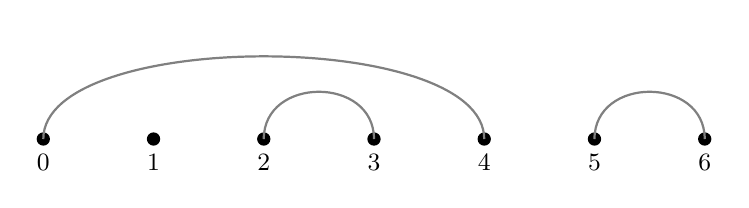
\begin{tikzpicture}[scale=1.0, baseline=(current bounding box.center)]
    \def\N{7}
    \def\DX{1.4}
    \def\Ybase{0}
    \foreach \i in {0,...,6} {
      \coordinate (P\i) at (\i*\DX,\Ybase);
      \fill (P\i) circle (2.4pt);
      \node[below=2pt, font=\small] at (P\i) {\i};
    }
    \draw[gray, thick] (P0) .. controls +(.0,1.4) and +(-.0,1.4) .. (P4);
    \draw[gray, thick] (P2) .. controls +(.0,0.8) and +(-.0,0.8) .. (P3);
    \draw[gray, thick] (P5) .. controls +(.0,0.8) and +(-.0,0.8) .. (P6);
  \end{tikzpicture}
  \caption{Example of an admissible composite move: arcs $(0,4)$, $(2,3)$, $(5,6)$.}
    \label{fig:motzkin_arcs}
\end{figure}

\subsection{Formal definition}
\paragraph{Swapping elements.} Given a permutation $\pi = (\pi_0,\pi_1,\ldots,\pi_{n-1})$ and a pair of indices $(i,j)$ satisfying $0 \le i < j < n$, we define the \emph{end swap} as the operation:
\begin{equation}\label{eq:S_ij}
S_{i,j}(\pi) = (\pi_0,\ldots,\pi_{i-1},\; \pi_j,\; \pi_{i+1},\ldots,\pi_{j-1},\; \pi_i,\; \pi_{j+1},\ldots,\pi_{n-1}).
\end{equation}
This operation swaps the elements indexed by $i$ and $j$, leaving the intermediate elements $\pi_{i+1},\ldots,\pi_{j-1}$ unchanged. Locally, the segment $[\pi_i,\pi_{i+1},\ldots,\pi_{j-1},\pi_j]$ is transformed into $[\pi_j,\pi_{i+1},\ldots,\pi_{j-1},\pi_i]$.

\paragraph{Composite move.} We define it as a set of index pairs $\mathcal{M} = \{(i_1,j_1), (i_2,j_2), \ldots, (i_k,j_k)\}$. The set $\mathcal{M}$ is \emph{admissible} if it satisfies the following conditions:

\begin{enumerate}
  \item \textbf{Index disjointness}: For any two index pairs $(i_a,j_a), (i_b,j_b) \in \mathcal{M}$ we have $\{i_a,j_a\} \cap \{i_b,j_b\} = \varnothing$ (no shared indices).
  
  \item \textbf{No crossings}: The pattern $i_a < i_b < j_a < j_b$ is forbidden for any $(i_a,j_a), (i_b,j_b) \in \mathcal{M}$ (arcs cannot intersect).
  
  \item \textbf{Nesting allowed}: The configuration $i_a < i_b < j_b < j_a$ is admissible (the inner pair is entirely contained within the outer pair).
\end{enumerate}


\subsection{Algorithm for constructing a new permutation}
The algorithm determines the set of pairs $\mathcal{M}$ within a single iteration. The goal is to construct a permutation $\pi$ that leads to makespan minimization.

\begin{enumerate}
  \item Determine the prefix completion columns $F[k][r]$.
  \item Compute $\Delta_{i,j}$ for all pairs $(i,j)$.
  \item Fill the table $\mathrm{dp}[L][R]$.
  \item Reconstruct the selected set of pairs $\mathcal{M}$.
  \item Apply the determined swaps to the permutation $\pi$.
\end{enumerate}


\section{Full Enumeration of Motzkin Composite Moves}
In the further part of the chapter we determine the number of admissible composite moves for a given $n$, and then we compare it with the Motzkin numbers $M_n$ corresponding to the same value of $n$.

\begin{table}[ht]
  \centering
  \caption{The first Motzkin numbers ($n=0..10$).}
  \begin{tabular}{@{}rcccccccccccc@{}}
    \toprule
    $n$ & 0 & 1 & 2 & 3 & 4 & 5 & 6 & 7 & 8 & 9 & 10 \\
    \midrule
    $M_n$ & 1 & 1 & 2 & 4 & 9 & 21 & 51 & 127 & 323 & 835 & 2188 \\
    \bottomrule
  \end{tabular}
\end{table}
 
\paragraph{Enumeration of Composite Moves for $n=0$.} There are no indices. Only the empty configuration exists.
\begin{enumerate}
  \item $\mathcal{M}_1 = \varnothing$.
\end{enumerate}
Verification: $1 = M_0$. \quad $\checkmark$

\paragraph{Enumeration of Composite Moves for $n=1$.} There is only one index (index 0), so the only admissible configuration is the empty set.
\begin{enumerate}
  \item $\mathcal{M}_1 = \varnothing$. \quad (index 0 isolated)
\end{enumerate}
Verification: $1 = M_1$. \quad $\checkmark$

\paragraph{Enumeration of Composite Moves for $n=2$.} We have two indices: 0 and 1. \\
Category I: Empty Composite Move:
\begin{enumerate}
  \item $\mathcal{M}_1 = \varnothing$. \quad (both indices isolated)
\end{enumerate}
Category II: One Pair:
\begin{enumerate}
  \setcounter{enumi}{1}
  \item $\mathcal{M}_2 = \{(0,1)\}$.
\end{enumerate}
Verification: $1 + 1 = 2 = M_2$. \quad $\checkmark$

\paragraph{Enumeration of Composite Moves for $n=3$.} We have three indices: 0, 1, 2.
Category I: Empty Composite Move
\begin{enumerate}
  \item $\mathcal{M}_1 = \varnothing$.
\end{enumerate}
Category II: One Pair:
\begin{multicols}{3}
\begin{enumerate}
  \setcounter{enumi}{1}
  \item $\mathcal{M}_2 = \{(0,1)\}$,
  \item $\mathcal{M}_3 = \{(0,2)\}$,
  \item $\mathcal{M}_4 = \{(1,2)\}$.
\end{enumerate}
\end{multicols}
Verification: $1 + 3 = 4 = M_3$. \quad $\checkmark$
Note: For $n=3$ it is not possible to form two disjoint pairs (this requires at least 4 indices).

\paragraph{Enumeration of Composite Moves for $n=4$.} We have four indices: 0, 1, 2, 3.
Category I: Empty Composite Move:
\begin{enumerate}
  \item $\mathcal{M}_1 = \varnothing$.
\end{enumerate}
Category II: One Pair:
\begin{multicols}{3}
\begin{enumerate}
  \setcounter{enumi}{1}
  \item $\mathcal{M}_2 = \{(0,1)\}$,
  \item $\mathcal{M}_3 = \{(0,2)\}$,
  \item $\mathcal{M}_4 = \{(0,3)\}$,
  \item $\mathcal{M}_5 = \{(1,2)\}$,
  \item $\mathcal{M}_6 = \{(1,3)\}$,
  \item $\mathcal{M}_7 = \{(2,3)\}$.
\end{enumerate}
\end{multicols}
Category III: Two Disjoint Pairs:
\begin{enumerate}
  \setcounter{enumi}{7}
  \item $\mathcal{M}_8 = \{(0,1), (2,3)\}$.
\end{enumerate}
Category IV: Two Nested Pairs:
\begin{enumerate}
  \setcounter{enumi}{8}
  \item $\mathcal{M}_9 = \{(0,3), (1,2)\}$.
\end{enumerate}
Verification: $1 + 6 + 1 + 1 = 9 = M_4$. \quad $\checkmark$

\paragraph{Enumeration of Composite Moves for $n=5$.} We have five indices: 0, 1, 2, 3, 4.
Category I: Empty Composite Move:
\begin{enumerate}
  \item $\mathcal{M}_1 = \varnothing$.
\end{enumerate}
Category II: One Pair:
\begin{multicols}{3}
\begin{enumerate}
  \setcounter{enumi}{1}
  \item $\mathcal{M}_2 = \{(0,1)\}$,
  \item $\mathcal{M}_3 = \{(0,2)\}$,
  \item $\mathcal{M}_4 = \{(0,3)\}$,
  \item $\mathcal{M}_5 = \{(0,4)\}$,
  \item $\mathcal{M}_6 = \{(1,2)\}$,
  \item $\mathcal{M}_7 = \{(1,3)\}$,
  \item $\mathcal{M}_8 = \{(1,4)\}$,
  \item $\mathcal{M}_9 = \{(2,3)\}$,
  \item $\mathcal{M}_{10} = \{(2,4)\}$,
  \item $\mathcal{M}_{11} = \{(3,4)\}$.
\end{enumerate}
\end{multicols}

Category III: Two Disjoint Pairs:
\begin{multicols}{2}
\begin{enumerate}
  \setcounter{enumi}{11}
  \item $\mathcal{M}_{12} = \{(0,1), (2,3)\}$,
  \item $\mathcal{M}_{13} = \{(0,1), (2,4)\}$,
  \item $\mathcal{M}_{14} = \{(0,1), (3,4)\}$,
  \item $\mathcal{M}_{15} = \{(0,2), (3,4)\}$,
  \item $\mathcal{M}_{16} = \{(1,2), (3,4)\}$,
\end{enumerate}
\end{multicols}

Category IV: Two Nested Pairs:
\begin{multicols}{2}
\begin{enumerate}
  \setcounter{enumi}{16}
  \item $\mathcal{M}_{17} = \{(0,3), (1,2)\}$,
  \item $\mathcal{M}_{18} = \{(0,4), (1,2)\}$,
  \item $\mathcal{M}_{19} = \{(0,4), (1,3)\}$,
  \item $\mathcal{M}_{20} = \{(0,4), (2,3)\}$,
  \item $\mathcal{M}_{21} = \{(1,4), (2,3)\}$.
\end{enumerate}
\end{multicols}
Verification: $1 + 10 + 5 + 5 = 21 = M_5$. \quad $\checkmark$

\paragraph{Enumeration of Composite Moves for $n=6$.} We have six indices: 0, 1, 2, 3, 4, 5. According to theory $M_6 = 51$.
Category I: Empty Composite Move:
\begin{enumerate}
  \item $\mathcal{M}_1 = \varnothing$.
\end{enumerate}
Category II: One Pair. All $\binom{6}{2} = 15$ pairs:
\begin{multicols}{3}
\begin{enumerate}
  \setcounter{enumi}{1}
  \item $\mathcal{M}_2 = \{(0,1)\}$,
  \item $\mathcal{M}_3 = \{(0,2)\}$,
  \item $\mathcal{M}_4 = \{(0,3)\}$,
  \item $\mathcal{M}_5 = \{(0,4)\}$,
  \item $\mathcal{M}_6 = \{(0,5)\}$,
  \item $\mathcal{M}_7 = \{(1,2)\}$,
  \item $\mathcal{M}_8 = \{(1,3)\}$,
  \item $\mathcal{M}_9 = \{(1,4)\}$,
  \item $\mathcal{M}_{10} = \{(1,5)\}$,
  \item $\mathcal{M}_{11} = \{(2,3)\}$,
  \item $\mathcal{M}_{12} = \{(2,4)\}$,
  \item $\mathcal{M}_{13} = \{(2,5)\}$,
  \item $\mathcal{M}_{14} = \{(3,4)\}$,
  \item $\mathcal{M}_{15} = \{(3,5)\}$,
  \item $\mathcal{M}_{16} = \{(4,5)\}$.
\end{enumerate}
\end{multicols}
Category III: Two Disjoint Pairs, $(i_1,j_1)$, $(i_2,j_2)$ with $j_1 < i_2$:
\begin{multicols}{2}
\begin{enumerate}
  \setcounter{enumi}{16}
  \item $\mathcal{M}_{17} = \{(0,1), (2,3)\}$,
  \item $\mathcal{M}_{18} = \{(0,1), (2,4)\}$,
  \item $\mathcal{M}_{19} = \{(0,1), (2,5)\}$,
  \item $\mathcal{M}_{20} = \{(0,1), (3,4)\}$,
  \item $\mathcal{M}_{21} = \{(0,1), (3,5)\}$,
  \item $\mathcal{M}_{22} = \{(0,1), (4,5)\}$,
  \item $\mathcal{M}_{23} = \{(0,2), (3,4)\}$,
  \item $\mathcal{M}_{24} = \{(0,2), (3,5)\}$,
  \item $\mathcal{M}_{25} = \{(0,2), (4,5)\}$,
  \item $\mathcal{M}_{26} = \{(0,3), (4,5)\}$,
  \item $\mathcal{M}_{27} = \{(1,2), (3,4)\}$,
  \item $\mathcal{M}_{28} = \{(1,2), (3,5)\}$,
  \item $\mathcal{M}_{29} = \{(1,2), (4,5)\}$,
  \item $\mathcal{M}_{30} = \{(1,3), (4,5)\}$,
  \item $\mathcal{M}_{31} = \{(2,3), (4,5)\}$.
\end{enumerate}
\end{multicols}
Category IV: Two Nested Pairs. Structure $i_a < i_b < j_b < j_a$:
\begin{multicols}{2}
\begin{enumerate}
  \setcounter{enumi}{31}
  \item $\mathcal{M}_{32} = \{(0,3), (1,2)\}$,
  \item $\mathcal{M}_{33} = \{(0,4), (1,2)\}$,
  \item $\mathcal{M}_{34} = \{(0,4), (1,3)\}$,
  \item $\mathcal{M}_{35} = \{(0,4), (2,3)\}$,
  \item $\mathcal{M}_{36} = \{(0,5), (1,2)\}$,
  \item $\mathcal{M}_{37} = \{(0,5), (1,3)\}$,
  \item $\mathcal{M}_{38} = \{(0,5), (1,4)\}$,
  \item $\mathcal{M}_{39} = \{(0,5), (2,3)\}$,
  \item $\mathcal{M}_{40} = \{(0,5), (2,4)\}$,
  \item $\mathcal{M}_{41} = \{(0,5), (3,4)\}$,
  \item $\mathcal{M}_{42} = \{(1,4), (2,3)\}$,
  \item $\mathcal{M}_{43} = \{(1,5), (2,3)\}$,
  \item $\mathcal{M}_{44} = \{(1,5), (2,4)\}$,
  \item $\mathcal{M}_{45} = \{(1,5), (3,4)\}$,
  \item $\mathcal{M}_{46} = \{(2,5), (3,4)\}$.
\end{enumerate}
\end{multicols}
Category V: Three Disjoint Pairs:
\begin{enumerate}
  \setcounter{enumi}{46}
  \item $\mathcal{M}_{47} = \{(0,1), (2,3), (4,5)\}$.
\end{enumerate}
Category VI: Two Disjoint + One Nested:
\begin{multicols}{2}
\begin{enumerate}
  \setcounter{enumi}{47}
  \item $\mathcal{M}_{48} = \{(0,3), (1,2), (4,5)\}$,
  \item $\mathcal{M}_{49} = \{(0,1), (2,5), (3,4)\}$.
\end{enumerate}
\end{multicols}
Category VII: Three Double-Nested Pairs:
\begin{enumerate}
  \setcounter{enumi}{49}
  \item $\mathcal{M}_{50} = \{(0,5), (1,4), (2,3)\}$.
\end{enumerate}
Category VIII: Mixed Structure
\begin{enumerate}
  \setcounter{enumi}{50}
  \item $\mathcal{M}_{51} = \{(0,5), (1,2), (3,4)\}$.
\end{enumerate}
Verification: $1 + 15 + 15 + 15 + 1 + 2 + 1 + 1 = 51 = M_6$. \quad $\checkmark$

\paragraph{Structure of Composite Moves for $n=7$.} We have $M_7 = 127$ configurations. Full enumeration would take many pages, so we present the combinatorial structure.
Main Categories:
\begin{itemize}
    \item Empty configuration: 1 element.
    \item One pair: $\binom{7}{2} = 21$ elements.
    \item Two disjoint pairs: We choose 4 indices out of 7 and split them into two pairs: $\binom{7}{4} \cdot \frac{1}{2}\binom{4}{2} = 35 \cdot 3 = 105$ elements. But we must exclude crossings. The correct number of disjoint pairs (without crossings): 35 elements.
    \item Two nested pairs: We choose an outer pair $(i,j)$ with span $\ge 3$, then an inner pair from $\{i+1, \ldots, j-1\}$: 35 elements.
    \item Three pairs: Combinations of three pairs (all disjoint or with nestings): 21 elements.
    \item Four or more pairs: Deeply nested structures and complex combinations: 14 elements.
\end{itemize}
Verification: $1 + 21 + 35 + 35 + 21 + 14 = 127 = M_7$. \quad $\checkmark$

\paragraph{Structure of Composite Moves for $n=8$.} Here $M_8 = 323$ configurations.
\\
Category distribution
\begin{multicols}{2}
\begin{itemize}
  \item Empty: 1.
  \item One pair: $\binom{8}{2} = 28$.
  \item Two pairs: $ 126$ (disjoint + nested).
  \item Three pairs: $ 112$.
  \item Four pairs: $ 51$.
  \item More pairs: $ 5$.
\end{itemize}
\end{multicols}
Verification by recurrence:
\begin{equation}
M_8 = M_7 + \sum_{k=0}^{6} M_k M_{6-k} = 127 + 196 = 323. \quad \checkmark
\end{equation}

\paragraph{Structure of Composite Moves for $n=9$.}
For $n=9$ we have $M_9 = 835$ configurations.
\\
Category distribution:
\begin{multicols}{2}
\begin{itemize}
  \item Empty: 1.
  \item One pair: $\binom{9}{2} = 36$.
  \item Two pairs: $ 330$.
  \item Three pairs: $ 294$.
  \item Four pairs: $ 140$.
  \item Five or more: $ 34$.
\end{itemize}
\end{multicols}
Verification by recurrence:
\begin{equation}
M_9 = M_8 + \sum_{k=0}^{7} M_k M_{7-k} = 323 + 512 = 835. \quad \checkmark 
\end{equation}

\paragraph{Structure of Composite Moves for $n=10$.} Here $M_{10} = 2188$ configurations.
\\
Category distribution (approximate)
\begin{multicols}{2}
\begin{itemize}
  \item Empty: 1.
  \item One pair: $\binom{10}{2} = 45$.
  \item Two pairs: $ 825$.
  \item Three pairs: $ 770$.
  \item Four pairs: $ 385$.
  \item Five pairs: $ 126$.
  \item More pairs: $ 36$.
\end{itemize}
\end{multicols}
Verification by recurrence:
\begin{equation}
M_{10} = M_9 + \sum_{k=0}^{8} M_k M_{8-k} = 835 + 1353 = 2188. \quad \checkmark 
\end{equation}

\paragraph{Remarks on Combinatorial Growth.}
For $n \ge 7$ the number of configurations grows exponentially ($M_n \sim c \cdot 3^n / n^{3/2}$), which makes full enumeration impractical. Despite this, the algorithm using dynamic programming remains efficient, running in time $O(n^3)$, without requiring explicit generation of all configurations -- the recurrence naturally searches the state space.

The bijection with Motzkin objects remains of key importance for understanding the theoretical structure, despite the lack of explicitly listing all $M_n$ composite moves.


\section{Experimental Setup}
The experiment was conducted in the test environment defined in \cite{WojewodzkiBozejko2026}, as follows. All experiments were conducted on a MacBook Pro with an M4 Pro processor, 24~GB of RAM, running macOS 26.0.1 (25A362) and Python~3.11.

\paragraph{Benchmarks}
Taillard instances \cite{ref_taillard} of varying $(n,m)$ (e.g., $n\in\{50,100,200,500\}$, $m\in\{10,20\}$). Each run is constrained by a wall-clock time budget (e.g., 100 ms). Seeds are fixed for reproducibility.

\paragraph{Parameters}
The following parameter values were used in the experiments:
\begin{itemize}
  \item Tabu tenure: $10$
  \item SA: $T_{\text{init}}=1000$, $T_{\text{final}}=1$, $\alpha=0.95$, reheating factor $r = 1.5$, stagnation threshold $500$ (ms).
\end{itemize}

\paragraph{Metrics}
\begin{itemize}
  \item Best $C_{\max}$ vs. time.
  \item Convergence curves (multi-neighborhood overlay).
  \item Effective moves per second (normalized).
  \item Plateau detection latency.
\end{itemize}
The choice of experimental parameters and metrics was primarily aimed at assessing the impact of the different neighborhood structures on the final solution quality, rather than evaluating the absolute performance of the algorithms.


\section{Results and Discussion}
\begin{figure*}[t]
  \centering

  \begin{subfigure}[t]{0.49\textwidth}
    \centering
    \includegraphics[width=\linewidth]{figures/gap_vs_time_tabu.png}
    \caption{Tabu Search}
    \label{fig:gap-vs-time-tabu-sub}
  \end{subfigure}\hfill
  \begin{subfigure}[t]{0.49\textwidth}
    \centering
    \includegraphics[width=\linewidth]{figures/gap_vs_time_sa.png}
    \caption{Simulated Annealing}
    \label{fig:gap-vs-time-sa-sub}
  \end{subfigure}
  \caption{Comparison of solution quality (mean gap to the lower bound, LB) as a function of the time limit for two metaheuristics and four neighborhoods.}
  \label{fig:gap-vs-time-both}
\end{figure*}


\begin{figure*}[t]
  \centering

  \begin{subfigure}[t]{0.49\textwidth}
    \centering
    \includegraphics[width=\linewidth]{figures/algo=sa_file=tai100_20_inst=3_tl=500ms_n100_m20_multi_1.png}
    \caption{Tabu Search, t=500ms, n=100, m=20}
    \label{fig:tabu_500_100_20}
  \end{subfigure}\hfill
  \begin{subfigure}[t]{0.49\textwidth}
    \centering
    \includegraphics[width=\linewidth]{figures/algo=tabu_file=tai200_10_inst=2_tl=2000ms_n200_m10_multi_1.png}
    \caption{Simulated Annealing, t=2000ms, n=200, m=10}
    \label{fig:sa_2000_200_10}
  \end{subfigure}
  \caption{Example graphs for individual algorithm runs.}
  \label{fig:example_results}
\end{figure*}

The results presented in Tables~\ref{tab:results_tl100}--\ref{tab:results_tl10000} and in the plots of the mean gap as a function of the time limit (Fig.~\ref{fig:gap-vs-time-both}) indicate that the choice of the neighborhood structure has a key impact on the final performance of the algorithm as a function of time. The averaged results indicate that, for all analyzed time limits, the ranking of neighborhoods is, in principle, similar. \emph{Dynasearch} has the lowest gap values. It is optimized computationally, which allows for performing a larger number of iterations within the same computation time. Additionally, for large datasets, a single \emph{Dynasearch} iteration takes much more time than the overall time limit. It should be noted that the time-limit condition was checked at the beginning of each algorithm iteration. After the limit was exceeded, it was still possible to finish the already started iteration and include its outcome. Therefore, in some cases the reported results correspond to an effective computation time that exceeds the nominal time limit. This allows us to omit the results for this neighborhood in the further part. In contrast, the \emph{Fibonacci} neighborhood performs the least favorably over the entire examined range. At the same time, in Fig.~\ref{fig:gap-vs-time-both} we observe a systematic improvement in solution quality with increasing $T_{\text{limit}}$. The rate of change depends on the applied neighborhood. For some of the applied methods, a rapid transition to the plateau phase is observed, which is visible in Fig.~\ref{fig:sa_2000_200_10}. This indicates the occurrence of a saturation effect and limits the possibility of further searching for better solutions.
The \emph{Motzkin} neighborhood is relatively large, but it allows for performing many swaps during a single iteration in a strictly structured manner. On average, this approach outperforms the \emph{Adjacent} neighborhood. This advantage becomes more visible for larger time limits, which suggests an advantage of multi-swap moves requiring sufficiently large time over simpler solutions. A natural direction for further research is an attempt to improve the computational efficiency of the implementations of the \emph{Motzkin} and \emph{Fibonacci} neighborhoods in order to increase the number of iterations that can be performed within the same time constraint. For the purpose of increasing the competitiveness of the new neighborhoods with respect to the classical ones.





\begin{table}[H]
\centering

\begin{minipage}{0.85\linewidth}
\centering
\resizebox{\linewidth}{!}{\small
\begin{tabular}{lccS[table-format=2.2]S[table-format=2.2]S[table-format=2.2]S[table-format=2.2]S[table-format=2.2]S[table-format=2.2]S[table-format=2.2]S[table-format=2.2]}
\multicolumn{11}{c}{\textbf{Time limit:} $tl_{\mathrm{ms}}=100$} \\ 
\hline
\textbf{file} & {$n$} & {$m$} & {adj$_{\mathrm{TABU}}$} & {adj$_{\mathrm{SA}}$} & {fib$_{\mathrm{TABU}}$} & {fib$_{\mathrm{SA}}$} & {dyn$_{\mathrm{TABU}}$} & {dyn$_{\mathrm{SA}}$} & {mot$_{\mathrm{TABU}}$} & {mot$_{\mathrm{SA}}$} \\ 
\hline
tai100\_10 & 100 & 10 & 18.41 & 19.62 & {\bfseries 17.34} & {\bfseries 17.34} & 17.33 & 17.33 & 18.98 & 18.98 \\ 
tai100\_20 & 100 & 20 & 27.55 & 27.94 & {\bfseries 24.50} & {\bfseries 24.50} & 25.50 & 25.50 & 27.20 & 27.20 \\ 
tai100\_5 & 100 & 5 & 11.84 & 11.98 & {\bfseries 11.15} & {\bfseries 11.15} & 11.01 & 11.01 & 12.48 & 12.25 \\ 
tai200\_10 & 200 & 10 & 15.40 & 15.28 & {\bfseries 14.01} & {\bfseries 14.01} & 13.20 & 13.20 & 14.79 & 14.79 \\ 
tai200\_20 & 200 & 20 & 23.26 & 23.33 & {\bfseries 21.62} & {\bfseries 21.62} & 20.71 & 20.71 & 22.06 & 22.06 \\ 
tai20\_10 & 20 & 10 & 19.59 & 20.73 & 29.73 & 29.73 & 14.68 & 14.68 & {\bfseries 16.61} & 17.61 \\ 
tai20\_20 & 20 & 20 & 31.89 & 30.30 & 36.37 & 36.37 & 24.83 & 24.83 & {\bfseries 25.56} & 25.58 \\ 
tai20\_5 & 20 & 5 & {\bfseries 7.18} & 7.98 & 17.39 & 17.39 & 6.18 & 6.18 & 8.39 & 8.39 \\ 
tai500\_20 & 500 & 20 & 16.25 & 16.03 & {\bfseries 15.57} & {\bfseries 15.57} & 14.51 & 14.51 & 15.93 & 15.93 \\ 
tai50\_10 & 50 & 10 & {\bfseries 19.65} & 22.10 & 20.23 & 20.23 & 16.84 & 17.00 & 19.86 & 20.17 \\ 
tai50\_20 & 50 & 20 & 32.54 & 34.23 & 32.19 & 32.23 & 31.14 & 31.14 & {\bfseries 30.57} & {\bfseries 30.57} \\ 
tai50\_5 & 50 & 5 & 10.71 & {\bfseries 8.38} & 12.13 & 12.13 & 6.20 & 6.07 & 10.35 & 10.45 \\ 
AVG &  &  & 19.52 & 19.82 & 21.02 & 21.02 & 16.84 & 16.85 & 18.57 & 18.66 \\ 
\hline
\end{tabular}
}
\caption{Average results for $T_{\text{limit}} = 100$ ms.}
\label{tab:results_tl100}
\end{minipage}

\vspace{1em}

\begin{minipage}{0.85\linewidth}
\centering
\resizebox{\linewidth}{!}{\small
\begin{tabular}{lccS[table-format=2.2]S[table-format=2.2]S[table-format=2.2]S[table-format=2.2]S[table-format=2.2]S[table-format=2.2]S[table-format=2.2]S[table-format=2.2]}
\multicolumn{11}{c}{\textbf{Time limit:} $tl_{\mathrm{ms}}=500$} \\ 
\hline
\textbf{file} & {$n$} & {$m$} & {adj$_{\mathrm{TABU}}$} & {adj$_{\mathrm{SA}}$} & {fib$_{\mathrm{TABU}}$} & {fib$_{\mathrm{SA}}$} & {dyn$_{\mathrm{TABU}}$} & {dyn$_{\mathrm{SA}}$} & {mot$_{\mathrm{TABU}}$} & {mot$_{\mathrm{SA}}$} \\ 
\hline
tai100\_10 & 100 & 10 & {\bfseries 16.92} & 17.16 & 17.19 & 17.19 & 15.69 & 16.08 & 17.22 & 17.51 \\ 
tai100\_20 & 100 & 20 & 24.98 & 26.33 & {\bfseries 23.02} & {\bfseries 23.02} & 25.50 & 25.50 & 26.30 & 26.30 \\ 
tai100\_5 & 100 & 5 & 10.89 & {\bfseries 6.65} & 11.15 & 11.15 & 8.73 & 8.73 & 11.99 & 11.99 \\ 
tai200\_10 & 200 & 10 & 14.10 & 14.72 & {\bfseries 12.72} & {\bfseries 12.72} & 13.20 & 13.20 & 14.79 & 14.79 \\ 
tai200\_20 & 200 & 20 & 22.09 & 22.80 & {\bfseries 19.74} & 19.76 & 20.71 & 20.71 & 22.06 & 22.06 \\ 
tai20\_10 & 20 & 10 & {\bfseries 14.91} & 20.37 & 29.73 & 29.73 & 14.68 & 14.68 & 16.61 & 17.61 \\ 
tai20\_20 & 20 & 20 & 27.35 & 30.22 & 36.37 & 36.37 & 24.83 & 24.83 & {\bfseries 25.49} & {\bfseries 25.49} \\ 
tai20\_5 & 20 & 5 & {\bfseries 5.23} & 6.52 & 17.39 & 17.39 & 6.18 & 6.18 & 8.39 & 8.39 \\ 
tai500\_20 & 500 & 20 & 16.09 & 16.00 & {\bfseries 15.13} & {\bfseries 15.13} & 14.51 & 14.51 & 15.93 & 15.93 \\ 
tai50\_10 & 50 & 10 & 17.97 & {\bfseries 12.63} & 20.23 & 20.23 & 9.94 & 9.94 & 16.77 & 16.77 \\ 
tai50\_20 & 50 & 20 & 30.51 & 26.72 & 32.19 & 32.19 & 23.31 & 23.31 & 25.70 & {\bfseries 25.64} \\ 
tai50\_5 & 50 & 5 & 10.22 & {\bfseries 3.54} & 12.13 & 12.13 & 2.95 & 2.95 & 8.31 & 8.92 \\ 
AVG &  &  & 17.61 & 16.97 & 20.58 & 20.58 & 15.02 & 15.05 & 17.46 & 17.62 \\ 
\hline
\end{tabular}
}
\caption{Average results for $T_{\text{limit}} = 500$ ms.}
\label{tab:results_tl500}
\end{minipage}

\vspace{1em}

\begin{minipage}{0.85\linewidth}
\centering
\resizebox{\linewidth}{!}{\small
\begin{tabular}{lccS[table-format=2.2]S[table-format=2.2]S[table-format=2.2]S[table-format=2.2]S[table-format=2.2]S[table-format=2.2]S[table-format=2.2]S[table-format=2.2]}
\multicolumn{11}{c}{\textbf{Time limit:} $tl_{\mathrm{ms}}=1000$} \\ 
\hline
\textbf{file} & {$n$} & {$m$} & {adj$_{\mathrm{TABU}}$} & {adj$_{\mathrm{SA}}$} & {fib$_{\mathrm{TABU}}$} & {fib$_{\mathrm{SA}}$} & {dyn$_{\mathrm{TABU}}$} & {dyn$_{\mathrm{SA}}$} & {mot$_{\mathrm{TABU}}$} & {mot$_{\mathrm{SA}}$} \\ 
\hline
tai100\_10 & 100 & 10 & 16.68 & {\bfseries 12.14} & 17.19 & 17.19 & 14.03 & 14.08 & 16.35 & 16.42 \\ 
tai100\_20 & 100 & 20 & 24.06 & 25.41 & {\bfseries 23.02} & {\bfseries 23.02} & 23.43 & 23.43 & 24.51 & 24.51 \\ 
tai100\_5 & 100 & 5 & 10.83 & {\bfseries 4.43} & 11.15 & 11.15 & 7.04 & 7.04 & 11.53 & 11.53 \\ 
tai200\_10 & 200 & 10 & 13.44 & 14.36 & {\bfseries 12.71} & {\bfseries 12.71} & 13.20 & 13.20 & 14.79 & 14.79 \\ 
tai200\_20 & 200 & 20 & 21.44 & 22.49 & {\bfseries 19.11} & {\bfseries 19.11} & 20.71 & 20.71 & 22.06 & 22.06 \\ 
tai20\_10 & 20 & 10 & {\bfseries 13.34} & 20.25 & 29.73 & 29.73 & 14.68 & 14.68 & 16.61 & 17.61 \\ 
tai20\_20 & 20 & 20 & 25.75 & 30.22 & 36.37 & 36.37 & 24.83 & 24.83 & {\bfseries 25.49} & {\bfseries 25.49} \\ 
tai20\_5 & 20 & 5 & {\bfseries 4.76} & 6.31 & 17.39 & 17.39 & 6.18 & 6.18 & 8.39 & 8.39 \\ 
tai500\_20 & 500 & 20 & 15.96 & 15.93 & {\bfseries 14.94} & {\bfseries 14.94} & 14.51 & 14.51 & 15.93 & 15.93 \\ 
tai50\_10 & 50 & 10 & 17.78 & {\bfseries 11.81} & 20.23 & 20.23 & 7.46 & 7.46 & 16.29 & 16.35 \\ 
tai50\_20 & 50 & 20 & 29.31 & 24.92 & 32.19 & 32.19 & 20.25 & 20.22 & {\bfseries 23.62} & 23.96 \\ 
tai50\_5 & 50 & 5 & 9.84 & {\bfseries 2.44} & 12.13 & 12.13 & 2.95 & 2.95 & 8.06 & 8.52 \\ 
AVG &  &  & 16.93 & 15.89 & 20.51 & 20.51 & 14.11 & 14.11 & 16.97 & 17.13 \\ 
\hline
\end{tabular}
}
\caption{Average results for $T_{\text{limit}} = 1000$ ms.}
\label{tab:results_tl1000}
\end{minipage}

\end{table}

\begin{table}[H]
\centering

\begin{minipage}{0.85\linewidth}
\centering
\resizebox{\linewidth}{!}{\small
\begin{tabular}{lccS[table-format=2.2]S[table-format=2.2]S[table-format=2.2]S[table-format=2.2]S[table-format=2.2]S[table-format=2.2]S[table-format=2.2]S[table-format=2.2]}
\multicolumn{11}{c}{\textbf{Time limit:} $tl_{\mathrm{ms}}=2000$} \\ 
\hline
\textbf{file} & {$n$} & {$m$} & {adj$_{\mathrm{TABU}}$} & {adj$_{\mathrm{SA}}$} & {fib$_{\mathrm{TABU}}$} & {fib$_{\mathrm{SA}}$} & {dyn$_{\mathrm{TABU}}$} & {dyn$_{\mathrm{SA}}$} & {mot$_{\mathrm{TABU}}$} & {mot$_{\mathrm{SA}}$} \\ 
\hline
tai100\_10 & 100 & 10 & 16.53 & {\bfseries 9.63} & 17.19 & 17.19 & 11.19 & 11.10 & 15.47 & 15.54 \\ 
tai100\_20 & 100 & 20 & 23.61 & {\bfseries 19.84} & 23.02 & 23.02 & 21.31 & 21.31 & 23.38 & 23.85 \\ 
tai100\_5 & 100 & 5 & 10.81 & {\bfseries 3.41} & 11.15 & 11.15 & 4.83 & 4.78 & 11.41 & 11.41 \\ 
tai200\_10 & 200 & 10 & 13.27 & 13.77 & {\bfseries 12.71} & {\bfseries 12.71} & 13.20 & 13.20 & 14.35 & 14.35 \\ 
tai200\_20 & 200 & 20 & 20.70 & 21.80 & {\bfseries 18.65} & {\bfseries 18.65} & 20.71 & 20.71 & 22.06 & 22.06 \\ 
tai20\_10 & 20 & 10 & {\bfseries 12.92} & 19.80 & 29.73 & 29.73 & 14.68 & 14.68 & 16.61 & 17.61 \\ 
tai20\_20 & 20 & 20 & {\bfseries 24.74} & 30.22 & 36.37 & 36.37 & 24.83 & 24.83 & 25.49 & 25.49 \\ 
tai20\_5 & 20 & 5 & {\bfseries 4.40} & 6.31 & 17.39 & 17.39 & 6.18 & 6.18 & 8.39 & 8.39 \\ 
tai500\_20 & 500 & 20 & 15.75 & 15.91 & {\bfseries 14.48} & {\bfseries 14.48} & 14.51 & 14.51 & 15.93 & 15.93 \\ 
tai50\_10 & 50 & 10 & 17.33 & {\bfseries 10.94} & 20.23 & 20.23 & 6.95 & 6.95 & 14.52 & 16.35 \\ 
tai50\_20 & 50 & 20 & 28.43 & 24.63 & 32.19 & 32.19 & 16.65 & 16.69 & {\bfseries 22.86} & 23.62 \\ 
tai50\_5 & 50 & 5 & 9.80 & {\bfseries 1.96} & 12.13 & 12.13 & 2.95 & 2.95 & 8.06 & 8.52 \\ 
AVG &  &  & 16.52 & 14.85 & 20.44 & 20.44 & 13.17 & 13.16 & 16.54 & 16.93 \\ 
\hline
\end{tabular}
}
\caption{Average results for $T_{\text{limit}} = 2000$ ms.}
\label{tab:results_tl2000}
\end{minipage}

\vspace{1em}

\begin{minipage}{0.85\linewidth}
\centering
\resizebox{\linewidth}{!}{\small
\begin{tabular}{lccS[table-format=2.2]S[table-format=2.2]S[table-format=2.2]S[table-format=2.2]S[table-format=2.2]S[table-format=2.2]S[table-format=2.2]S[table-format=2.2]}
\multicolumn{11}{c}{\textbf{Time limit:} $tl_{\mathrm{ms}}=5000$} \\ 
\hline
\textbf{file} & {$n$} & {$m$} & {adj$_{\mathrm{TABU}}$} & {adj$_{\mathrm{SA}}$} & {fib$_{\mathrm{TABU}}$} & {fib$_{\mathrm{SA}}$} & {dyn$_{\mathrm{TABU}}$} & {dyn$_{\mathrm{SA}}$} & {mot$_{\mathrm{TABU}}$} & {mot$_{\mathrm{SA}}$} \\ 
\hline
tai100\_10 & 100 & 10 & 16.52 & {\bfseries 8.31} & 17.19 & 17.19 & 6.48 & 6.57 & 14.32 & 14.82 \\ 
tai100\_20 & 100 & 20 & 23.22 & {\bfseries 17.52} & 23.02 & 23.02 & 17.62 & 17.62 & 21.75 & 21.92 \\ 
tai100\_5 & 100 & 5 & 10.72 & {\bfseries 2.40} & 11.15 & 11.15 & 2.34 & 2.34 & 9.22 & 10.73 \\ 
tai200\_10 & 200 & 10 & 13.19 & {\bfseries 8.51} & 12.71 & 12.71 & 13.20 & 13.20 & 14.07 & 14.26 \\ 
tai200\_20 & 200 & 20 & 19.83 & 20.18 & {\bfseries 18.60} & {\bfseries 18.60} & 20.71 & 20.71 & 20.42 & 20.85 \\ 
tai20\_10 & 20 & 10 & {\bfseries 12.58} & 19.58 & 29.73 & 29.73 & 14.68 & 14.68 & 16.61 & 17.61 \\ 
tai20\_20 & 20 & 20 & {\bfseries 22.61} & 30.16 & 36.37 & 36.37 & 24.83 & 24.83 & 25.49 & 25.49 \\ 
tai20\_5 & 20 & 5 & {\bfseries 4.17} & 6.24 & 17.39 & 17.39 & 6.18 & 6.18 & 8.39 & 8.39 \\ 
tai500\_20 & 500 & 20 & 15.35 & 15.82 & 13.93 & {\bfseries 13.91} & 14.51 & 14.51 & 15.93 & 15.93 \\ 
tai50\_10 & 50 & 10 & 17.10 & {\bfseries 9.71} & 20.23 & 20.23 & 6.95 & 6.95 & 13.35 & 16.35 \\ 
tai50\_20 & 50 & 20 & 27.65 & 24.44 & 32.19 & 32.19 & 14.80 & 14.84 & {\bfseries 20.95} & 23.44 \\ 
tai50\_5 & 50 & 5 & 9.38 & {\bfseries 1.96} & 12.13 & 12.13 & 2.95 & 2.95 & 8.06 & 8.52 \\ 
AVG &  &  & 16.03 & 13.74 & 20.39 & 20.39 & 12.10 & 12.12 & 15.71 & 16.53 \\ 
\hline
\end{tabular}
}
\caption{Average results for $T_{\text{limit}} = 5000$ ms.}
\label{tab:results_tl5000}
\end{minipage}

\vspace{1em}

\begin{minipage}{0.85\linewidth}
\centering
\resizebox{\linewidth}{!}{\small
\begin{tabular}{lccS[table-format=2.2]S[table-format=2.2]S[table-format=2.2]S[table-format=2.2]S[table-format=2.2]S[table-format=2.2]S[table-format=2.2]S[table-format=2.2]}
\multicolumn{11}{c}{\textbf{Time limit:} $tl_{\mathrm{ms}}=10000$} \\ 
\hline
\textbf{file} & {$n$} & {$m$} & {adj$_{\mathrm{TABU}}$} & {adj$_{\mathrm{SA}}$} & {fib$_{\mathrm{TABU}}$} & {fib$_{\mathrm{SA}}$} & {dyn$_{\mathrm{TABU}}$} & {dyn$_{\mathrm{SA}}$} & {mot$_{\mathrm{TABU}}$} & {mot$_{\mathrm{SA}}$} \\ 
\hline
tai100\_10 & 100 & 10 & 16.50 & {\bfseries 6.19} & 17.19 & 17.19 & 4.11 & 4.11 & 13.58 & 14.40 \\ 
tai100\_20 & 100 & 20 & 22.92 & {\bfseries 17.06} & 23.02 & 23.02 & 15.50 & 15.50 & 19.87 & 20.69 \\ 
tai100\_5 & 100 & 5 & 10.57 & {\bfseries 2.37} & 11.15 & 11.15 & 1.93 & 1.93 & 8.38 & 10.73 \\ 
tai200\_10 & 200 & 10 & 13.16 & {\bfseries 7.23} & 12.71 & 12.71 & 11.66 & 11.66 & 14.07 & 14.07 \\ 
tai200\_20 & 200 & 20 & 19.63 & {\bfseries 14.61} & 18.60 & 18.60 & 19.32 & 19.32 & 20.17 & 20.17 \\ 
tai20\_10 & 20 & 10 & {\bfseries 12.07} & 19.58 & 29.73 & 29.73 & 14.68 & 14.68 & 16.61 & 17.61 \\ 
tai20\_20 & 20 & 20 & {\bfseries 22.12} & 30.16 & 36.37 & 36.37 & 24.83 & 24.83 & 25.49 & 25.49 \\ 
tai20\_5 & 20 & 5 & {\bfseries 4.04} & 6.24 & 17.39 & 17.39 & 6.18 & 6.18 & 8.39 & 8.39 \\ 
tai500\_20 & 500 & 20 & 14.98 & 15.53 & {\bfseries 13.62} & {\bfseries 13.62} & 14.51 & 14.51 & 15.93 & 15.93 \\ 
tai50\_10 & 50 & 10 & 17.10 & {\bfseries 9.06} & 20.23 & 20.23 & 6.95 & 6.95 & 13.35 & 16.35 \\ 
tai50\_20 & 50 & 20 & 26.58 & 24.32 & 32.19 & 32.19 & 14.73 & 14.80 & {\bfseries 20.37} & 23.44 \\ 
tai50\_5 & 50 & 5 & 9.38 & {\bfseries 1.81} & 12.13 & 12.13 & 2.95 & 2.95 & 8.06 & 8.52 \\ 
AVG &  &  & 15.75 & 12.85 & 20.36 & 20.36 & 11.45 & 11.45 & 15.36 & 16.32 \\ 
\hline
\end{tabular}
}
\caption{Average results for $T_{\text{limit}} = 10000$ ms.}
\label{tab:results_tl10000}
\end{minipage}

\end{table}




\bibliographystyle{splncs04}
\bibliography{mybibliography}


\end{document}
